\normalfalse \difficiletrue \tdifficilefalse
\correctiontrue

%\UPSTIidClasse{11} % 11 sup, 12 spé
%\newcommand{\UPSTIidClasse}{12}

\exer{Mouvement RT -- RSG  $\star\star$ \label{B2:13:09}}
\setcounter{question}{0}\marginnote{\UPSTIcompetence[2]{B2-13}}
\index{Compétence B2-13}
\index{Mécanisme à 1 rotations, 1 translation et RSG}
\ifcorrection
\else
\marginnote{\textbf{Pas de corrigé pour cet exercice.}}
\fi

\ifprof
\else
Soit le mécanisme suivant. On a $\vect{IA}=R\vect{j_0}$ et $\vect{AB}=\lambda(t)\vect{i_1}$. De plus $R=\SI{15}{mm}$.
On fait l'hypothèse de roulement sans glissement au point $I$.
\begin{center}
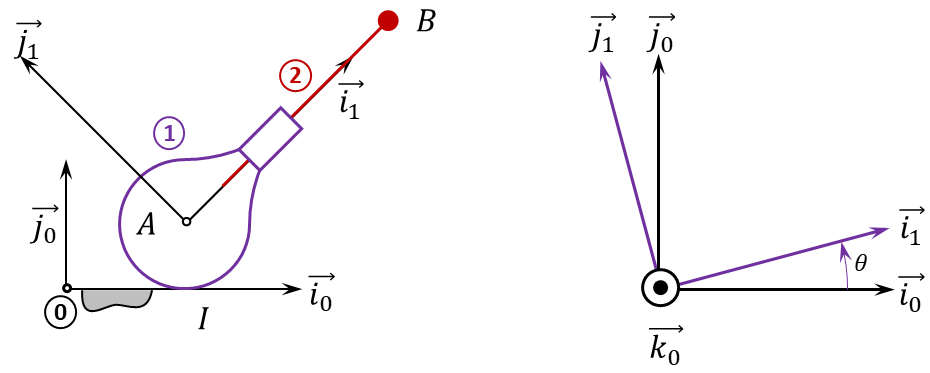
\includegraphics[width=\linewidth]{09_RT_RSG_01}
\end{center}
\fi


\question{Déterminer $\vectv{B}{2}{0}$.}
\ifprof ~\\
$\vectv{B}{2}{0}=\vectv{B}{2}{1}+\vectv{B}{1}{0}$.

D'une part,  $\vectv{B}{2}{1}=\lambdap\vi{1}$.

D'autre part, en utilisant le roulement sans glissement en $I$, 
$\babarv{B}{I}{1}{0} $ $=\vect{0}+\left(-\lambda(t)\vi{1}-R\vj{0} \right)\wedge\thetap \vk{0}$
$=-\thetap\left(\lambda(t)\vi{1}\wedge \vk{0}+R\vj{0}\wedge \vk{0} \right)$
$=\thetap\left(\lambda(t)\vj{1}-R\vi{0} \right)$.

Au final, $\vectv{B}{2}{0} = \lambdap\vi{1} + \thetap\left(\lambda(t)\vj{1}-R\vi{0} \right)$.

\else
\fi

\question{Donner le torseur cinématique $\torseurcin{V}{2}{0}$ au point $B$.}
\ifprof ~\\
$\torseurcin{V}{2}{0}=\torseurl{\thetap \vk{0}}{ \lambdap\vi{1} + \thetap\left(\lambda(t)\vj{1}-R\vi{0} \right)}{B}$.
\else
\fi

\question{Déterminer $\vectg{B}{2}{0}$.}
\ifprof ~\\
$\vectg{B}{2}{0} = \deriv{\vectv{B}{2}{0}}{\rep{0}}$
$ = \lambdapp(t)\vi{1} +\lambdap(t)\thetap\vj{1} 
+ \thetapp(t)\left(\lambda(t)\vj{1}-R\vi{0} \right)
+ \thetap(t)\left(\lambdap(t)\vj{1}-\lambda(t)\thetap\vi{1} \right)
$.
\else
\fi

\ifprof
\else
\ifcolle
\else
\begin{solution}
\begin{enumerate}
\item $\vectv{B}{2}{0} = \lambdap\vi{1} + \thetap\left(\lambda(t)\vj{1}-R\vi{0} \right)$.
\item $\torseurcin{V}{2}{0}=\torseurl{\thetap \vk{0}}{ \lambdap\vi{1} + \thetap\left(\lambda(t)\vj{1}-R\vi{0} \right)}{B}$.
\item $\vectg{B}{2}{0}  = \lambdapp(t)\vi{1} +\lambdap(t)\thetap\vj{1} 
+ \thetapp(t)\left(\lambda(t)\vj{1}-R\vi{0} \right)
+ \thetap(t)\left(\lambdap(t)\vj{1}-\lambda(t)\thetap\vi{1} \right)
$.
\end{enumerate} 
\end{solution}
\fi

\marginnote{Corrigé  voir \ref{B2:13:09}.}
\fi